\ifx\wholebook\relax\else
\documentclass{report}
\usepackage{times}
\usepackage{epsfig}
\usepackage{alltt}
\usepackage{xspace}
\usepackage{graphicx}
\usepackage{ifpdf}
\usepackage{ifthen}
\usepackage{amsmath}
\usepackage{a4wide}

\graphicspath{{figures/}} 

\ifpdf
\DeclareGraphicsExtensions{.pdf, .jpg, .tif, .png}
\else
\DeclareGraphicsExtensions{.eps, .jpg}
\fi

\newboolean{toseecomment}
\setboolean{toseecomment}{false}
%%change to false to hidde comment 
\newcommand{\comment}[1]{\ifthenelse{\boolean{toseecomment}}{$\blacktriangleright$ \textit{#1}$\blacktriangleleft$}{}}

\newcommand{\commented}[1]{}

\newboolean{seevwspecific}
\setboolean{seevwspecific}{true}
\newcommand{\vwspecific}[1]{\ifthenelse{\boolean{seevwspecific}}{#1}{}}

\newboolean{seecategoryspecific}
\setboolean{seecategoryspecific}{false}
\newcommand{\categoryspecific}[1]{\ifthenelse{\boolean{seecategoryspecific}}{#1}{}}

\newboolean{seestorespecific}
\setboolean{seestorespecific}{true}
\newcommand{\storespecific}[1]{\ifthenelse{\boolean{seestorespecific}}{#1}{}}

\newboolean{seesqueakspecific}
\setboolean{seesqueakspecific}{false}
\newcommand{\squeakspecific}[1]{\ifthenelse{\boolean{seesqueakspecific}}{#1}{}}


\newcommand{\category}[0]
{\ifthenelse{\boolean{seestorespecific}}
	{package\xspace}
	{category\xspace}}

\newcommand{\ct}[1]{\texttt{#1}\xspace}
\newcommand{\stc}[1]{{\small {\sf #1}}\xspace}
\newcommand{\ST}{{\textsc Smalltalk}\xspace}
\newcommand{\tab}{\makebox[4em]{}}
\newcommand{\ttt}[1]{{\tt #1}}
\newcommand{\chev}{\ttt{>>}}
\newcommand{\vw}{VisualWorks\xspace}
\newcommand{\sq}{Squeak\xspace}
\newcommand{\store}{Store\xspace}
\renewcommand{\chaptername}{Exercise}
\newcommand{\exercise}{\vspace{0.2cm}\noindent \textbf{Exercise:}\xspace}

\newsavebox{\fminibox}
\newlength{\fminilength}

% Fait un truc encadre
\newenvironment{fminipage}[1][\linewidth]
  {\setlength{\fminilength}{#1-2\fboxsep-2\fboxrule}
        \begin{lrbox}{\fminibox}\begin{minipage}{\fminilength}}
  { \end{minipage}\end{lrbox}\noindent\fbox{\usebox{\fminibox}}}

% Pareil mais pas encadre (a utiliser pour ne pas couper une fonction

\newenvironment{nminipage}[1][\linewidth]
  {\setlength{\fminilength}{#1}
        \begin{lrbox}{\fminibox}\begin{minipage}{\fminilength}}
  { \end{minipage}\end{lrbox}\noindent\mbox{\usebox{\fminibox}}}

% Un alltt encadre
\newenvironment{falltt}
  {\vspace*{0.3cm}\begin{fminipage}\begin{alltt}}
  {\end{alltt}\end{fminipage}\vspace*{0.3cm}}

% Un alltt pas encadre
\newenvironment{nalltt}
  {\vspace*{0.3cm}\begin{nminipage}\begin{alltt}}
  {\end{alltt}\end{nminipage}\vspace*{0.3cm}}

% Une fonction encadree
\newenvironment{ffonction}[1]
  {\begin{fonction}[#1]
        \begin{fminipage}
\begin{alltt}
\rule{\linewidth}{0.5pt}}
{\end{alltt}\end{fminipage}\end{fonction}}

\newenvironment{codeonepage}
  {\begin{nminipage}\vspace*{0.2cm}\hrule\vspace*{0.1cm}
\begin{alltt}}
  {\end{alltt} \vspace*{-0.2cm}\hrule \vspace*{0.2cm} \end{nminipage}}

\newenvironment{code}
  {\vspace*{0.1cm}\hrule\vspace*{-0.1cm}\begin{alltt}}
  {\end{alltt}\vspace*{-0.2cm}\hrule \vspace*{0.1cm}}


\begin{document}
\fi

% $Author: ducasse $
% $Date: 2005/05/16 13:38:19 $
% $Revision: 1.1.1.1 $


\chapter{Web dynamique avec Seaside}
\mainauthor{\bouraqadi}

\metadata{Squeak}{?Squeak/VisualWorks?}{?www.squeaksource.com/RegConf?}{?1.2?}{??}

%%%%%% %%%%%% %%%%%% %%%%%% %%%%%% %%%%%% %%%%%% %%%%%%
\section{Compl\'ements sur Seaside}


Quelques messages pour g\'en\'erer du html. Le destinataire de ces messages est l'objet pass\'e en param\`etre de la m\'ethode \ct{renderOn:} (instance de \ct{WAHtmlRender}). 

\begin{itemize}
\item \ct{text: 'chaine de caracteres'} affiche simplement la cha�ne de caract\`eres.
\item \ct{heading: 'texte du titre' level: niveau} affiche un titre. Le deuxi\`eme param\`etre est un entier qui correspond au niveau hi\'erarchique du titre (1 correspond au le plus grand)
\item \ct{break} introduit un retour \`a la ligne
\item \ct{horizontalRule} introduit une ligne horizontale
\item \ct{form: ["definition de boutons, zones de saisies, �"]} d\'efinit un formulaire au sens Html. N\'ecessaire pour avoir des boutons et autres zones de saisies dans une page Html. Re�oit en param\`etre un bloc qui contient les messages de cr\'eation des boutons, zones de saisie, �

\item \ct{textInputWithValue: valeurInitiale callback: [ :valeur \stBar "traitements"]} cr\'ee une zone de saisie simple (sans barre de d\'efilement). La valeur initiale est celle qui est affich\'ee au d\'emarrage (nil pour ne rien afficher). Le dernier argument est un bloc qui re\c coit comme param\`etre la valeur saisie (valeur) dans le champ. Cette valeur peut \^etre utilis\'ee dans le traitement d\'efini par le bloc. Ce bloc est ex\'ecut\'e quand la touche "Entr\'ee" est press\'ee ou quand on clic sur un bouton du formulaire dans lequel se trouve la zone de saisie.
\item \ct{submitButtonWitAction: ["traitements"] text: 'titre du bouton'} ajoute un bouton qui a pour titre la cha�ne de caract\`eres pass\'ee comme deuxi\`eme argument. Un clic sur le bouton provoque l'ex\'ecution des traitements d\'efinis dans le bloc pass\'e comme premier param\`etre.
\end{itemize}


\section{Encore des compteurs !}
Il s'agit de r\'ealiser encore un compteur, mais cette fois, il devra \^etre accessible via le web (utilisation de Seaside). De plus, il devra \^etre personnalisable dans la mesure o\`u l'utilisateur doit pouvoir modifier directement la valeur du compteur et modifier l'incr\'ement. Concr\`etement, vous devez d\'efinir une classe \ct{CompteurPersonnalise} sous-classe de \ct{WAComponent} qui repr\'esente une application Seaside. \ct{CompteurPersonnalise} sera munie de :

\begin{itemize}
\item deux champs (\ct{value} et \ct{increment}), 
\item une m\'ethode d'initialisation (\ct{initialize}),
\item ainsi que la m\'ethode de g\'en\'eration du code html (\ct{renderOn:}).
\end{itemize}

L'interface utilisateur doit \^etre analogue \`a celle de la figure~\ref{ExtendedCounter1}. Deux champs de saisie permettent de modifier la valeur du compteur et son incr\'ement apr\`es clic sur le bouton "Actualiser". Le bouton "Reset" r\'einitialise le compteur (\ct{value} mise \`a 0 et \ct{increment} mis \`a 1). Enfin, le bouton "Incr\'ementer/D\'ecr\'ementer" permet d'ajouter l'incr\'ement au compteur et donc de l'incr\'ementer si l'incr\'ement est positif ou de le d\'ecr\'ementer dans le cas contraire.
 
\begin{figure} 
\begin{center}
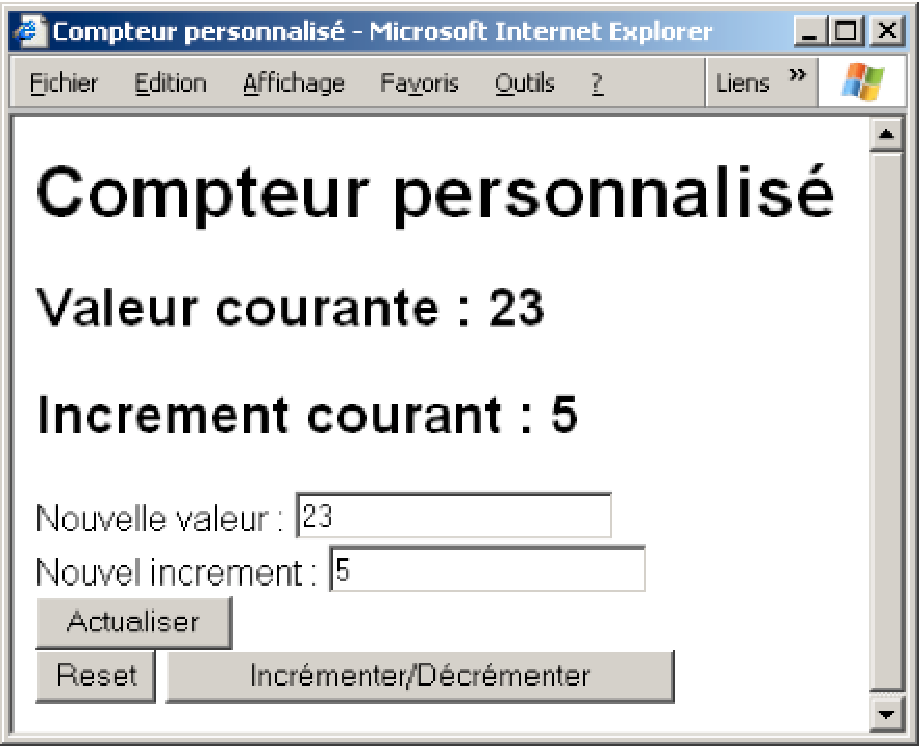
\includegraphics[width=8cm]{ExtendedCounter1}
\caption{L'interface du compteur personnalis\'e\label{ExtendedCounter1}}
\end{center}
\end{figure}


\section{S\'eparer l'interface du code m\'etier}
La structure sugg\'er\'ee pour l'exercice pr\'ec\'edent n'est pas tr\`es propre. En effet, un m\^eme objet prend en charge \`a la fois le traitement (code m\'etier : incr\'ementer/d\'ecr\'ementer, modification de l'incr\'ement, �) et l'interface utilisateur. Ce choix de conception rend difficile les \'eventuelles \'evolutions ou r\'eutilisation. En particulier, si l'on souhaite changer d'interface utilisateur, voire de mod\`ele de communication distante.

Dans cet exercice, on se propose de faire la s\'eparation entre code m\'etier et code d'interface et en illustrer l'utilit\'e \`a l'aide d'un exemple simple. Cet exemple tourne autour d'une calculatrice arithm\'etique. Vous d\'efinirez tout d'abord la classe \ct{Calculatrice} qui dispose de deux champs qui repr\'esentent respectivement l'op\'erande gauche et l'op\'erande droite. Munissez la classe d'accesseurs en lecture \'ecriture \`a ces deux champs, ainsi que de 4 m\'ethodes pour r\'ealiser les 4 op\'erations arithm\'etiques. Bien entendu, ces quatre m\'ethodes :
\begin{itemize}
\item ne prennent pas de param\`etres,
\item effectuent le calcul en utilisant les champs repr\'esentant les deux op\'erandes,
\item et retournent le r\'esultat du calcul 
\end{itemize}

D\'efinissez ensuite la classe \ct{CalculatriceWeb} sous-classe de \ct{WAComponent} qui repr\'esente une application Seaside. \ct{CalculatriceWeb} permet l'utilisation \`a travers le web des op\'erations fournies par \ct{Calculatrice}. Son interface s'apparente \`a celle donn\'ee par la figure~\ref{ExtendedCounter2}.


Vous allez maintenant exploiter la s\'eparation entre code m\'etier et code d'interface utilisateur. En effet, vous allez r\'eutiliser la classe \ct{Calculatrice} pour faire un nouveau compteur accessible via le web. L'interface devra \^etre identique \`a celle du compteur de l'exercice pr\'ec\'edent. 

\begin{figure} 
\begin{center}
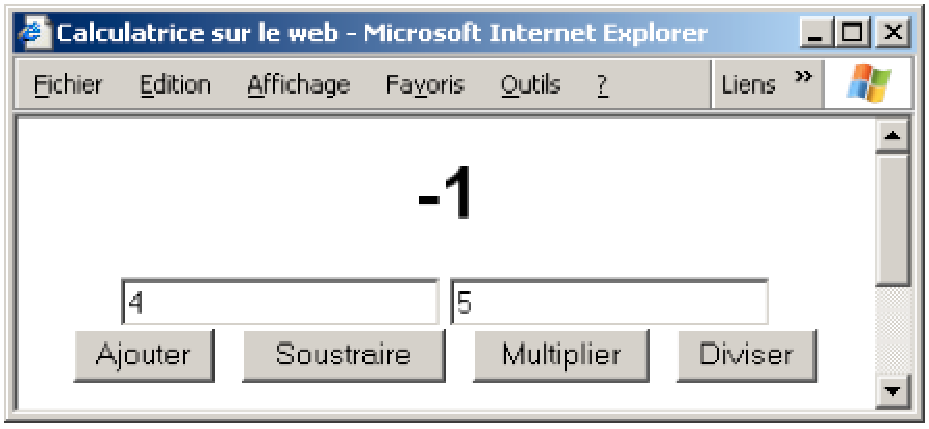
\includegraphics[width=8cm]{ExtendedCounter2}
\caption{L'interface de la calculatrice. \label{ExtendedCounter2}}
\end{center}
\end{figure}


\section{Une application un peu plus sophistiqu\'ee}
Il s'agit ici de d\'efinir un outil qui permet de g\'erer des tableaux blancs partag\'es via le web. Un tableau blanc est une zone de texte que plusieurs utilisateurs peuvent modifier. Chaque tableau est caract\'eris\'e par un nom et dispose d'une liste identifiants les utilisateurs qui ont le droit d'y acc\'eder.

Chaque utilisateur dispose d'un identifiant et d'un mot de passe qu'il fournit pour se connecter. Une fois connect\'e il a le choix entre cr\'eer un nouveau tableau ou modifier tableau existant.   Les utilisateurs qui ont acc\`es \`a un tableau peuvent en modifier le contenu ainsi que la liste des utilisateurs qui ont acc\`es au tableau.

\ifx\wholebook\relax\else\end{document}\fi

